\documentclass[../PianoDiProgetto.tex]{subfiles}
\begin{document}
\newpage
	\section{Preventivo}
		\subsection{Dettaglio fasi}
			\subsubsection{\PerAR}
				\paragraph{Suddivisione del lavoro}\
	\begin{table}[H]
		%\centering
		\begin{tabularx}{\textwidth}{l*{6}{c}c}
			\toprule
			\textbf{Nominativo} & \textbf{Rp} & \textbf{Am} & \textbf{Pt} 
						& \textbf{An} & \textbf{Pm} & \textbf{Ve} & \textbf{Ore totali} \\
			\midrule
			Andrea Magnan & 0 & 10 &	0 &	8 & 0 & 7 & 28 \\
			%\midrule
			Luca Bertolini & 3 & 7 & 0 & 0 & 0 & 17 & 27 \\
			%\midrule
			Mattia Bottaro &	0 &	10 & 0 & 7 & 0 & 10 & 27 \\
			%\midrule
			Mauro Carlin & 0 & 13 &	0 &	10 & 0 & 3 & 26 \\
			%\midrule
			Nicola Tintorri &	0 & 10 & 0 & 7 & 0 & 10 & 27 \\
			%\midrule
			Pier Paolo Tricomi & 8 & 3 &	0 &	13 & 0 & 4 & 28 \\
			%\midrule
			Simeone Pizzi & 11 & 4 & 0 & 14 & 0 & 0 & 26 \\
			\midrule			
			\textbf{Ore Totali Ruolo} & 22 & 57 & 0 & 59 &	0 &	51 & 189 \\
			\bottomrule
		\end{tabularx}
		\caption{\PerAR{} - Suddivisione delle ore di lavoro}
		%\label{tab:faseA_ore}
	\end{table}
	
	\vspace{15 mm}	
	
	\begin{figure}[H]
		\centering
		\includegraphics[width=11cm, trim=1cm 0cm 1cm 0cm]{grafici/AR-persona}
			\caption{\PerAR{} - Riassunto}
		%\label{fig:BarChart-faseA_ore}
	\end{figure}	
	
\newpage
	\vfill	
	\paragraph{Prospetto economico}\
	
	\begin{table}[H]
		\centering
		\begin{tabular}{l * {2}{c}}
			\toprule
			\textbf{Ruolo} & \textbf{Ore} & \textbf{Costo(\euro{})} \\
			\midrule
			Responsabile &	22 &  660,00 \\
			%\midrule
			Amministratore & 57 &  1.140,00 \\
			%\midrule
			Progettista & 0 & 0,00 \\
			%\midrule
			Analista & 59 & 1.475,00 \\
			%\midrule
			Programmatore & 0 & 0,00 \\
			%\midrule
			Verificatore & 51 & 765,00 \\
			\midrule		
			\textbf{Totale} & 189 & 4.040,00 \\
			\bottomrule	
		\end{tabular}
		\caption{\PerAR{} - Costo per ruolo}
		%\label{tab:faseA_costo}
	\end{table}

\vspace{35 mm}	

	\begin{figure}[H]
		\centering
		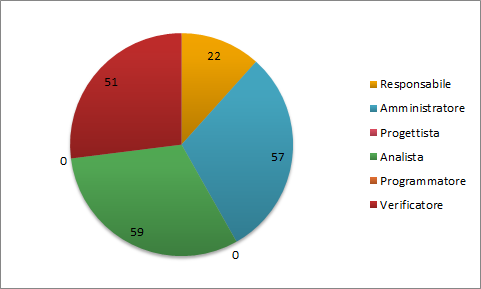
\includegraphics[width=11cm, trim=1cm 0cm 1cm 0cm]{grafici/AR-ruolo}
			\caption{\PerAR{} - Ore per ruolo}
		%\label{fig:CircleChart-faseA_ore_r}
	\end{figure}
	\vfill
	\newpage
	\vfill	
	\begin{figure}[H]
		\centering
		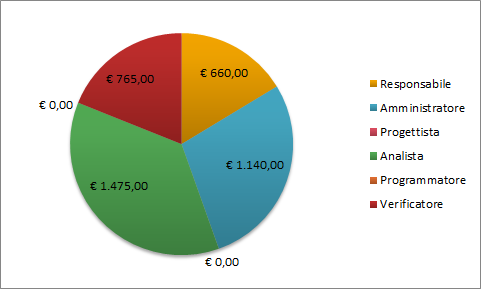
\includegraphics[width=11cm, trim=1cm 0cm 1cm 0cm]{grafici/AR-costo}
			\caption{\PerAR{} - Costo per ruolo}
		%\label{fig:CircleChart-faseA_costo}
	\end{figure}

\vspace{20 mm}
	
	\subsubsection{\PerAD}
				\paragraph{Suddivisione del lavoro}\
				
	\begin{table}[H]
		%\centering
		\begin{tabularx}{\textwidth}{l  * {6}{c}  c}
			\toprule
			\textbf{Nominativo} & \textbf{Rp} & \textbf{Am} & \textbf{Pt} 
						& \textbf{An} & \textbf{Pm} & \textbf{Ve} & \textbf{Ore totali} \\
			\midrule
			Andrea Magnan & 0 & 4 &	0 &	0 & 0 & 4 & 8 \\
			%\midrule
			Luca Bertolini & 0 & 4 & 0 & 0 & 0 & 4 & 8 \\
			%\midrule
			Mattia Bottaro & 0 & 0 & 0 & 4 & 0 & 4 & 8 \\
			%\midrule
			Mauro Carlin & 0 & 0 &	0 &	4 & 0 & 4 & 8 \\
			%\midrule
			Nicola Tintorri &	6 & 2 & 0 & 0 & 0 & 0 & 8 \\
			%\midrule
			Pier Paolo Tricomi & 0 & 0 &	0 &	3 & 0 & 5 & 8 \\
			%\midrule
			Simeone Pizzi & 0 & 0 & 0 & 3 & 0 & 5 & 8 \\
			\midrule			
			\textbf{Ore Totali Ruolo} & 6 & 10 & 0 & 14 & 0 & 26 & 56 \\
			\bottomrule
		\end{tabularx}	
		\caption{\PerAD{} - Suddivisione delle ore di lavoro}
		%\label{tab:faseAD_ore}	
	\end{table}
\newpage

	\vspace{15 mm}	
	
	
	\begin{figure}[H]
		\centering
		\includegraphics[width=11cm, trim=1cm 0cm 1cm 0cm]{grafici/AD-persona}
			\caption{\PerAD{} - Riassunto}
		%\label{fig:BarChart-faseAD_ore}
	\end{figure}
	
\vspace{35 mm}	
	
	\paragraph{Prospetto economico}\
	
					\begin{table}[H]
		\centering
	
		\begin{tabular}{l * {2}{c}}
			\toprule
			\textbf{Ruolo} & \textbf{Ore} & \textbf{Costo (\euro{})} \\
			\midrule
			Responsabile &	6 & 180,00 \\
			%\midrule
			Amministratore & 10 & 200,00 \\
			%\midrule
			Progettista & 0 & 0,00 \\
			%\midrule
			Analista & 14 & 350,00 \\
			%\midrule
			Programmatore & 0 & 0,00 \\
			%\midrule
			Verificatore & 26 & 390,00 \\
			\midrule		
			\textbf{Totale} & 56 & 1.120,00 \\
			\bottomrule 
		\end{tabular}
		\caption{\PerAD{} - Costo per ruolo}
		%\label{tab:faseAD_costo}
	\end{table}
\vfill
\newpage
	
	\begin{figure}[H]
		\centering
		\includegraphics[width=11cm, trim=1cm 0cm 1cm 0cm]{grafici/AD-ruolo}
			\caption{\PerAD{} - Ore per ruolo}
		%\label{fig:CircleChart-faseAD_ore_r}
	\end{figure}
\vfill
	\begin{figure}[H]
		\centering
		\includegraphics[width=11cm, trim=1cm 0cm 1cm 0cm]{grafici/AD-costo}
			\caption{\PerAD{} - Costo per ruolo}
		%\label{fig:CircleChart-faseAD_costo}
	\end{figure}
\vfill		
\newpage	
	\subsubsection{\PerPA}
				\paragraph{Suddivisione del lavoro}\
						
	\begin{table}[H]
		\centering
	
		\begin{tabularx}{\textwidth}{l  * {6}{c}  c}
			\toprule
			\textbf{Nominativo} & \textbf{Rp} & \textbf{Am} & \textbf{Pt} 
						& \textbf{An} & \textbf{Pm} & \textbf{Ve} & \textbf{Ore totali} \\
			\midrule
			Andrea Magnan  & 0 & 0 & 0 & 18 & 0 & 1 & 19 \\
			Luca Bertolini  & 0 & 0 & 0 & 12 & 0 & 5 & 17 \\
			Mattia Bottaro  & 7 & 0 & 0 & 9 & 0 & 0 & 16 \\
			Mauro Carlin  & 0 & 0 & 7 & 7 & 0 & 3 & 17 \\
			Nicola Tintorri  & 0 & 0 & 13 & 6 & 0 & 0 & 19 \\
			Pier Paolo Tricomi  & 0 & 7 & 6 & 0 & 0 & 4 & 17 \\
			Simeone Pizzi & 0 & 7 & 11 & 0 & 0 & 0 & 18 \\
			\midrule
			\textbf{Ore Totali Ruolo} & 7 & 14 & 37 & 52 & 0 & 13 & 123 \\
			\bottomrule
		\end{tabularx}
		\caption{\PerPA{} - Suddivisione delle ore di lavoro}
		%\label{tab:fasePA_ore}
	\end{table}
\vfill	
	
	\begin{figure}[H]
		\centering
		\includegraphics[width=11cm, trim=1cm 0cm 1cm 0cm]{grafici/PA-persona}
			\caption{\PerPA{} - Riassunto}
		%\label{fig:BarChart-fasePA_ore}
	\end{figure}
\vfill	
\newpage
	
	\paragraph{Prospetto economico}\
					
	\begin{table}[H]
		\centering
	
		\begin{tabular}{l * {2}{c}}
			\toprule
			\textbf{Ruolo} & \textbf{Ore} & \textbf{Costo (\euro{})} \\
			\midrule
			Responsabile & 7    & 210,00 \\
			Amministratore  & 14    & 280,00 \\
			Progettista  & 37    & 814,00 \\
			Analista & 52    & 1.300,00 \\
			Programmatore  & 0    & 0,00 \\
			Verificatore  & 13    & 195,00 \\
			\midrule
			\textbf{Totale}  & 123   & 2.799,00 \\
			\bottomrule
		\end{tabular}
		\caption{\PerPA{} - Costo per ruolo}
		%\label{tab:fasePA_costo}
	\end{table}
\vfill	
	
	\begin{figure}[H]
		\centering
		\includegraphics[width=11cm, trim=1cm 0cm 1cm 0cm]{grafici/PA-ruolo}
			\caption{\PerPA{} - Ore per ruolo}
		%\label{fig:CircleChart-fasePA_ore_r}
	\end{figure}
\vfill	
\newpage
\vfill
	\begin{figure}[H]
		\centering
		\includegraphics[width=11cm, trim=1cm 0cm 1cm 0cm]{grafici/PA-costo}
			\caption{\PerPA{} - Costo per ruolo}
		%\label{fig:CircleChart-fasePA_costo}
	\end{figure}	
\vfill	
	\subsubsection{\PerPD}
				\paragraph{Suddivisione del lavoro}\
					
	
	\begin{table}[H]
		%\centering
	
		\begin{tabularx}{\textwidth}{l  * {6}{c}  c}
			\toprule
			\textbf{Nominativo} & \textbf{Rp} & \textbf{Am} & \textbf{Pt} 
						& \textbf{An} & \textbf{Pm} & \textbf{Ve} & \textbf{Ore totali} \\
			\midrule
			Andrea Magnan  & 3 & 4 & 6 & 0 & 0 & 0 & 13 \\
			Luca Bertolini  & 6 & 0 & 4 & 2 & 0 & 2 & 14 \\
			Mattia Bottaro  & 0 & 0 & 2 & 5 & 0 & 8 & 15 \\
			Mauro Carlin  & 0 & 6 & 0 & 4 & 0 & 4 & 14 \\
			Nicola Tintorri  & 0 & 0 & 0 & 14 & 0 & 0 & 14 \\
			Pier Paolo Tricomi  & 0 & 0 & 3 & 10 & 0 & 0 & 13 \\
			Simeone Pizzi & 0 & 0 & 1 & 8 & 0 & 4 & 13 \\
			\midrule			
			\textbf{Ore Totali Ruolo}& 9 & 10 & 16 & 43 & 0 & 18 & 96 \\
			\bottomrule	
		\end{tabularx}
		\caption{\PerPD{} - Suddivisione delle ore di lavoro}
		
	\end{table}
\vfill
\newpage
\vfill	
		
	\begin{figure}[H]
		\centering
		\includegraphics[width=11cm, trim=1cm 0cm 1cm 0cm]{grafici/PD-persona}
			\caption{\PerPD{} - Riassunto}
		
	\end{figure}
\vfill	
	\paragraph{Prospetto economico}\
					
	\begin{table}[H]
		\centering
	
		\begin{tabular}{l * {2}{c}}
			\toprule
			\textbf{Ruolo} & \textbf{Ore} & \textbf{Costo (\euro{})} \\
			\midrule
			Responsabile & 9    &  270,00 \\
			Amministratore  & 10     &  200,00 \\
			Progettista  & 16    &  352,00 \\
			Analista & 43   &  1.075,00 \\
			Programmatore  & 0    &  0,00 \\
			Verificatore  & 18    &  270,00 \\
			\midrule
			\textbf{Totale}  & 96   &  2.167,00 \\
			\bottomrule		
		\end{tabular}
		\caption{\PerPD{} - Costo per ruolo}
		
	\end{table}
\vfill	
\newpage
\vfill
	
	\begin{figure}[H]
		\centering
		\includegraphics[width=11cm, trim=1cm 0cm 1cm 0cm]{grafici/PD-ruolo}
			\caption{\PerPD{}- Ore per ruolo}
		
	\end{figure}

\vfill	
	\begin{figure}[H]
		\centering
		\includegraphics[width=11cm, trim=1cm 0cm 1cm 0cm]{grafici/PD-costo}
			\caption{\PerPD{} - Costo per ruolo}
	\end{figure}
\vfill	
\newpage	
	
	\subsubsection{\PerC}
				\paragraph{Suddivisione del lavoro}\
						
	\begin{table}[H]
		%\centering
		\begin{tabularx}{\textwidth}{l  * {6}{c}  c}
			\toprule
			\textbf{Nominativo} & \textbf{Rp} & \textbf{Am} & \textbf{Pt} 
						& \textbf{An} & \textbf{Pm} & \textbf{Ve} & \textbf{Ore totali} \\
			\midrule
			Andrea Magnan  & 3 & 0 & 13 & 0 & 0 & 13 & 29 \\
			Luca Bertolini  & 0 & 6 & 12 & 0 & 9 & 0 & 27 \\
			Mattia Bottaro  & 0 & 9 & 10 & 0 & 8 & 0 & 27 \\
			Mauro Carlin  & 7 & 0 & 9 & 0 & 12 & 0 & 28 \\
			Nicola Tintorri  & 0 & 0 & 0 & 0 & 5 & 21 & 26 \\
			Pier Paolo Tricomi  & 0 & 0 & 8 & 0 & 12 & 7 & 27 \\
			Simeone Pizzi & 4 & 0 & 4 & 0 & 14 & 4 & 26 \\
			\midrule
			\textbf{Ore Totali Ruolo} & 14 & 15 & 56 & 0 & 60 & 45 & 190 \\
			\bottomrule
			
		\end{tabularx}
		\caption{\PerC{} - Suddivisione delle ore di lavoro}
	\end{table}
	
\vfill	
		
	\begin{figure}[H]
		\centering
		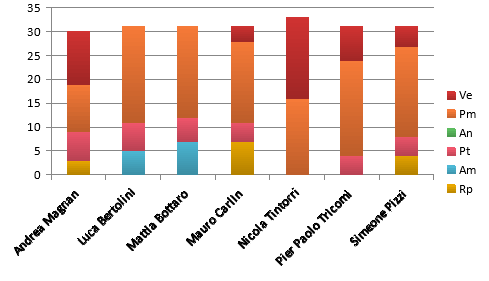
\includegraphics[width=11cm, trim=1cm 0cm 1cm 0cm]{grafici/C-persona}
			\caption{\PerC{}- Riassunto}
	\end{figure}
\vfill	
	
	\paragraph{Prospetto economico}\
					
	\begin{table}[H]
		\centering
	
		\begin{tabular}{l * {2}{c}}
			\toprule
			\textbf{Ruolo} & \textbf{Ore} & \textbf{Costo (\euro{})} \\
			\midrule
			Responsabile & 14    &  420,00 \\
			Amministratore  & 15    &  300,00 \\
			Progettista  & 56   &  1.232,00 \\
			Analista & 0    &  0,00 \\
			Programmatore  & 60    &  900,00 \\
			Verificatore  & 45    &  675,00 \\
			\midrule
			\textbf{Totale}  & 190   &  3.527,00 \\
			\bottomrule
		\end{tabular}
		\caption{\PerC{} - Costo per ruolo}
	\end{table}

\vspace{35mm}
	
	\begin{figure}[H]
		\centering
		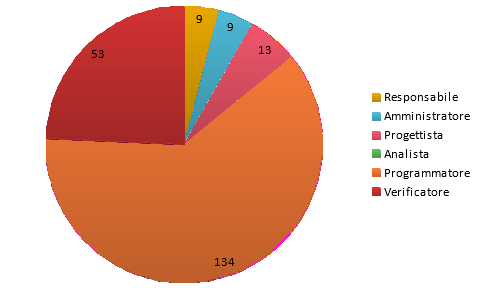
\includegraphics[width=11cm, trim=1cm 0cm 1cm 0cm]{grafici/C-ruolo}
			\caption{\PerC{} - Ore per ruolo}
	\end{figure}
\vfill
	\begin{figure}[H]
		\centering
		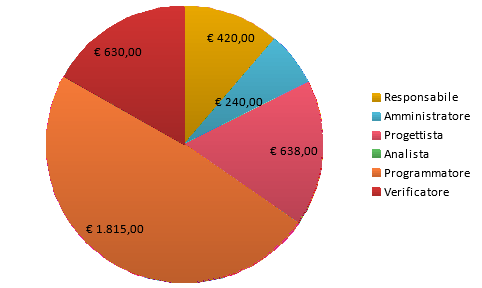
\includegraphics[width=11cm, trim=1cm 0cm 1cm 0cm]{grafici/C-costo}
			\caption{\PerC{} - Costo per ruolo}
	\end{figure}
	
\vspace{35mm}	
	
	
	\subsubsection{\PerV}
				\paragraph{Suddivisione del lavoro}\
					
	\begin{table}[H]
		%\centering
		\begin{tabularx}{\textwidth}{l  * {6}{c}  c}
			\toprule
			\textbf{Nominativo} & \textbf{Rp} & \textbf{Am} & \textbf{Pt} 
						& \textbf{An} & \textbf{Pm} & \textbf{Ve} & \textbf{Ore totali} \\
			\midrule
			Andrea Magnan  & 0 & 0 & 0 & 0 & 6 & 5 & 11 \\
			Luca Bertolini  & 0 & 0 & 0 & 0 & 8 & 4 & 12 \\
			Mattia Bottaro  & 0 & 0 & 5 & 0 & 0 & 7 & 12 \\
			Mauro Carlin  & 0 & 8 & 0 & 0 & 0 & 4 & 12 \\
			Nicola Tintorri  & 0 & 3 & 0 & 0 & 0 & 8 & 11 \\
			Pier Paolo Tricomi  & 7 & 0 & 0 & 0 & 4 & 1 & 12 \\
			Simeone Pizzi & 0 & 0 & 0 & 0 & 0 & 11 & 11 \\
			\midrule
			\textbf{Ore Totali Ruolo} & 7 & 11 & 5 & 0 & 18 & 40 & 81 \\
			\bottomrule
		\end{tabularx}
		\caption{\PerV{} - Suddivisione delle ore di lavoro}
	\end{table}
\vfill	

	
	\begin{figure}[H]
		\centering
		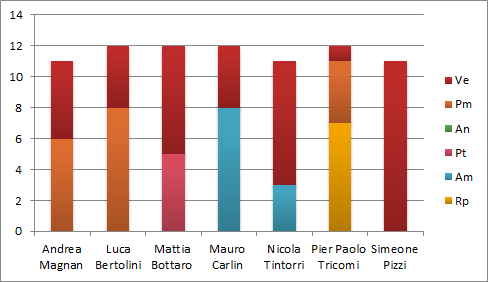
\includegraphics[width=11cm, trim=1cm 0cm 1cm 0cm]{grafici/V-persona}
			\caption{\PerV{} - Riassunto}
	\end{figure}
	
\vspace{35 mm}	
	\paragraph{Prospetto economico}\
					
	\begin{table}[H]
		\centering
	
		\begin{tabular}{l * {2}{c}}
			\toprule
			\textbf{Ruolo} & \textbf{Ore} & \textbf{Costo (\euro{})} \\
			\midrule
			Responsabile & 7 & 210,00 \\
			Amministratore  & 11 & 220,00 \\
			Progettista  & 5 & 110,00 \\
			Analista & 0 & 0,00 \\
			Programmatore  & 18 &  270,00 \\
			Verificatore  & 40 &  600,00 \\
			\midrule
			\textbf{Totale}  & 81   &  1.410,00 \\
			\bottomrule	
		\end{tabular}
		\caption{\PerV{} - Costo per ruolo}
	\end{table}
\vfill	
	
	\begin{figure}[H]
		\centering
		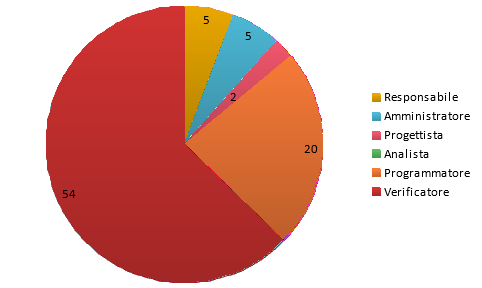
\includegraphics[width=11cm, trim=1cm 0cm 1cm 0cm]{grafici/V-ruolo}
			\caption{\PerV{} - Ore per ruolo}
	\end{figure}
\vfill	

	\begin{figure}[H]
		\centering
		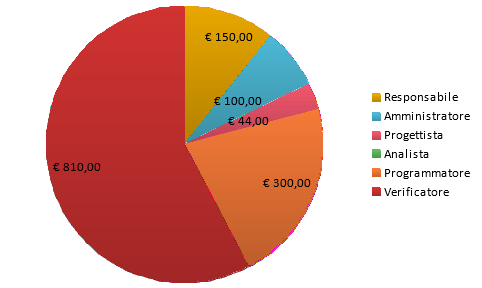
\includegraphics[width=11cm, trim=1cm 0cm 1cm 0cm]{grafici/V-costo}
			\caption{\PerV{} - Costo per ruolo}
	\end{figure}	
	
\vspace{35mm}	
	
	\subsection{Riepilogo}
			\subsubsection{Ore totali}
				\paragraph{Suddivisione del lavoro}\
					Le ore totali che ogni componente del gruppo \GRUPPO\ dedicherà ad ognuno dei ruoli, a rotazione, sono indicate di seguito:
	
	\begin{table}[H]
		%\centering
		\begin{tabularx}{\textwidth}{l  * {6}{c}  c}
			\toprule
			\textbf{Nominativo} & \textbf{Rp} & \textbf{Am} & \textbf{Pt} 
						& \textbf{An} & \textbf{Pm} & \textbf{Ve} & \textbf{Ore totali} \\
			\midrule
			Andrea Magnan  & 6  & 18 & 19 & 26 & 6  & 30 & 105 \\
			Luca Bertolini  & 9 & 17 & 16 & 14 & 17 & 32 & 105 \\
			Mattia Bottaro  & 7  & 19 & 17 & 25 & 8  & 29 & 105 \\
			Mauro Carlin  & 7 & 27 & 16 & 25 & 12 & 18 & 105 \\
			Nicola Tintorri  & 6 & 15 & 13 & 27 & 5 & 39 & 105 \\
			Pier Paolo Tricomi  & 15 & 10 & 17 & 26 & 16 & 21 & 105 \\
			Simeone Pizzi & 15 & 11 & 16 & 25 & 14 & 24 & 105 \\
			\midrule
			\textbf{Ore Totali Ruolo} & 65    & 117   & 114   & 168   & 78   & 193   & 735 \\
			\bottomrule
		\end{tabularx}
		\caption{Ore totali - Suddivisione delle ore di lavoro}
	\end{table}
	

\vfill
		
	\begin{figure}[H]
		\centering
		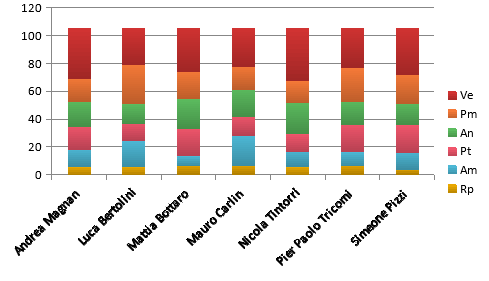
\includegraphics[width=11cm, trim=1cm 0cm 1cm 0cm]{grafici/TOT-persona}
			\caption{Ore persona totali - Riassunto}
		%\label{fig:BarChart-totale_ore}
	\end{figure}
	
\newpage	
	
	\paragraph{Prospetto economico}\
					Il costo totale per ogni ruolo è dunque il seguente:
	\begin{table}[H]
		\centering
		\begin{tabular}{l * {2}{c}}
			\toprule
			\textbf{Ruolo} & \textbf{Ore} & \textbf{Costo (\euro{})} \\
			\midrule
			Responsabile & 65    &  1.950,00 \\
			Amministratore  & 117   &  2.340,00 \\
			Progettista  & 114   &  2.508,00 \\
			Analista & 168   &  4.200,00 \\
			Programmatore  & 78   &  1.170,00 \\
			Verificatore  & 193   &  2.895,00 \\
			\midrule
			\textbf{Totale}  & 735  &  15.063,00 \\
			\bottomrule
			
		\end{tabular}
		\caption{Ore totali - Costo per ruolo}
		%\label{tab:totale_costo}
	\end{table}

\vspace{35 mm}	
	
	\begin{figure}[H]
		\centering
		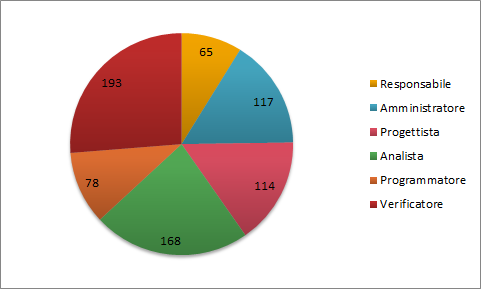
\includegraphics[width=11cm, trim=1cm 0cm 1cm 0cm]{grafici/TOT-ruolo}
			\caption{Ore totali - Ore per ruolo}
		%\label{fig:CircleChart-totale_ore_r}
	\end{figure}	
	
\newpage	
	
\vfill
	\begin{figure}[H]
		\centering
		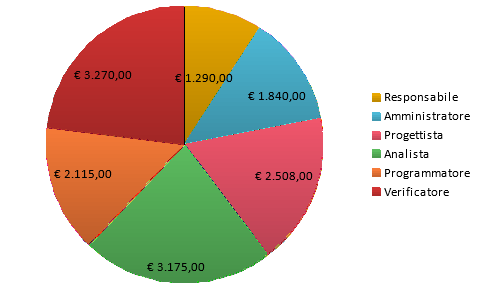
\includegraphics[width=11cm, trim=1cm 0cm 1cm 0cm]{grafici/TOT-costo}
			\caption{Ore totali - Costo per ruolo}
		%\label{fig:CircleChart-totale_ore}
	\end{figure}
\vfill
\newpage		
\end{document}